\section{Testing}

\begin{frame}[fragile]
    \frametitle{Test Environment}

    \begin{itemize}
        \item 프로세서 3.06GHz Intel Core 2 Duo, 메모리 4GB 
        \item \MM과 비교할 NFA 구현은 Perl 5.12를 사용
    \end{itemize}
    \begin{block}{Regular Expression Matcher in Perl}
    \small
    \begin{Verbatim}[xleftmargin=10mm]
use Time::HiRes qw( gettimeofday tv_interval );

for (my $ssize = 1; $ssize<=30; $ssize++) {
    my $str = 'a' x $ssize;
    my $pat = "(a?)\{$ssize\}a\{$ssize\}";

    my $t0 = [gettimeofday];
    # e.g. aaa =~ /(a?){3}a{3}/ when $ssize is 3
    $str =~ /$pat/;
    my $elapsed = tv_interval ( $t0 );

    print "$ssize,$elapsed\n";
}
    \end{Verbatim}
    \end{block}

\end{frame}

\begin{frame}
    \frametitle{Test Results}

NFA 기반의 정규 표현식 구현은 backtracking이 많은 경우에는 치명적인
성능 문제를 일으킬 잠재적인 위험이 있다.

우리의 구현 \MM은 backtracking이 없기 때문에 입력값의 길이에 선형적으로
비례하는 수행 시간을 보여 준다.

\[
    \rmatch{a}{a?a},  \rmatch{aa}{a?a?aa}, \dots,
    \rmatch{a^{30}}{(a?)^{30}a^{30}}
\]

\begin{figure}
\begin{columns}[b]
    \column{.5\paperwidth}
        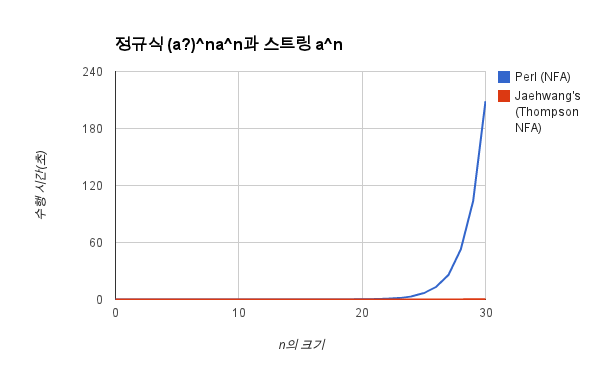
\includegraphics[width=.5\paperwidth]{result-compare.png}
    \column{.5\paperwidth}
        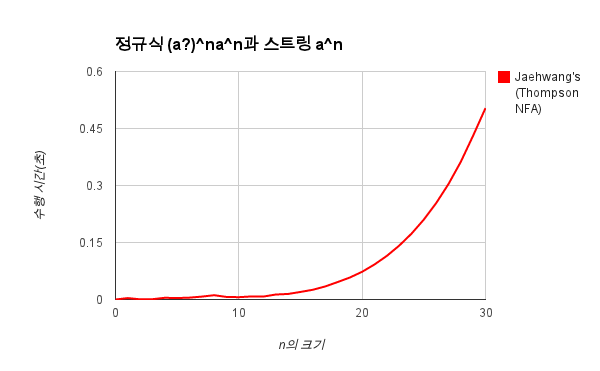
\includegraphics[width=.5\paperwidth]{result-single.png}
\end{columns}
\caption{왼쪽은 Perl과 \MM의 결과를 함께 보여주고, 오른쪽은 \MM의
    결과만 보여준다.}
\end{figure}
 
\end{frame}
